%%%%%%%%%%%%%%%%%%%%%%%%%%%%%%%%%%%%%%%%%
% Template ini dibuat untuk makalah seminar mahasiswa
% Program Alih Jenis (Ekstensi) Ilmu Komputer IPB
% Version 1.0 (18/05/2015)
%
% Template ini menggunakan template yang di-download dari:
% http://www.LaTeXTemplates.com
% Mathias Legrand (legrand.mathias@gmail.com)
% License: CC BY-NC-SA 3.0 (http://creativecommons.org/licenses/by-nc-sa/3.0/)
%
% Dimodifikasi untuk keperluan Program Studi
% Oleh: JULIO ADISANTOSO (julioipb@gmail.com)
%
% Untuk memudahkan penggunaan, maka diambil contoh makalah atas nama 
% Luthfi Noviandi di bawah bimbingan Julio Adisantoso ILKOM-IPB.
% Silakan mengganti dan melengkapi file:
%    (1) seminar_information.tex -- judul, nama, nim, email, pembimbing, dsb
%    (2) abstrak.tex -- abstrak makalah
%    (3) pendahuluan.tex -- berisi latar belakang, dsb
%    (4) metode.tex -- berisi metode penelitian
%    (5) hasil.tex -- berisi hasil dan pembahasan
%    (6) daftar_pustaka.tex -- berisi daftar pustaka
%
%%%%%%%%%%%%%%%%%%%%%%%%%%%%%%%%%%%%%%%%%

%----------------------------------------------------------------------------------------
%	PACKAGES AND OTHER DOCUMENT CONFIGURATIONS
%----------------------------------------------------------------------------------------

\documentclass[fleqn,11pt]{SelfArx} % Document font size and equations flushed left
\usepackage[english]{babel}

%----------------------------------------------------------------------------------------
%	COLUMNS
%----------------------------------------------------------------------------------------

\setlength{\columnsep}{0.55cm} % Distance between the two columns of text
\setlength{\fboxrule}{0.75pt} % Width of the border around the abstract

%----------------------------------------------------------------------------------------
%	COLORS
%----------------------------------------------------------------------------------------

\definecolor{color1}{RGB}{0,0,90} % Color of the article title and sections
\definecolor{color2}{RGB}{0,20,20} % Color of the boxes behind the abstract and headings

%----------------------------------------------------------------------------------------
%	HYPERLINKS
%----------------------------------------------------------------------------------------

\usepackage{hyperref} % Required for hyperlinks
\hypersetup{hidelinks,colorlinks,breaklinks=true,urlcolor=color2,citecolor=color1,linkcolor=color1,bookmarksopen=false,pdftitle={Title},pdfauthor={Author}}


%
% Hyphenation untuk Indonesia 
%
% @author  Andreas Febrian
% @version 1.00
% 
% Tambahkan cara pemenggalan kata-kata yang salah dipenggal secara otomatis 
% oleh LaTeX. Jika kata tersebut dapat dipenggal dengan benar, maka tidak 
% perlu ditambahkan dalam berkas ini. Tanda pemenggalan kata menggunakan 
% tanda '-'; contoh: menarik  --> pemenggalan: me-na-rik
%

\hyphenation{
    % alphabhet A
    a-na-li-sa a-tur 
    a-pli-ka-si 
    % alphabhet B
    ba-ngun-an 
    be-be-ra-pa 
    ber-ge-rak
    ber-ke-lan-jut-an 
    ber-pe-nga-ruh 
    % alphabhet C
    ca-ri
    % alphabhet D
    di-sim-pan di-pim-pin de-ngan da-e-rah di-ba-ngun da-pat di-nya-ta-kan 
    di-sim-bol-kan di-pi-lih di-li-hat de-fi-ni-si di-kem-bang-kan di-be-ri-kan
    % alphabhet E
    e-ner-gi eks-klu-sif
    % alphabhet F
    fa-si-li-tas
    % alphabhet G
    ga-bung-an ge-rak
    % alphabhet H
    ha-lang-an
    % alphabhet I
    % alphabhet J
    jang-krik
    % alphabhet K
    ke-hi-lang-an
    ku-ning 
    kua-li-tas ka-me-ra ke-mung-kin-an ke-se-pa-ham-an
    % alphabhet L
    ling-kung-an
    % alphabhet M
    me-neng-ah
    meng-a-tas-i me-mung-kin-kan me-nge-na-i me-ngi-rim-kan 
    meng-u-bah meng-a-dap-ta-si me-nya-ta-kan mo-di-fi-ka-si
    meng-a-tur meng-um-pul-kan meng-hi-tam-kan
    % alphabhet N
    nya-ta non-eks-klu-sif
    % alphabhet O
    % alphabhet P
	pe-nye-rap-an 
	pe-ngon-trol
    pe-mo-del-an
    pe-ran  pe-ran-an-nya
    pem-ba-ngun-an pre-si-den pe-me-rin-tah prio-ri-tas peng-am-bil-an 
    peng-ga-bung-an pe-nga-was-an pe-ngem-bang-an 
    pe-nga-ruh pa-ra-lel-is-me per-hi-tung-an per-ma-sa-lah-an 
    pen-ca-ri-an peng-struk-tur-an
    % alphabhet Q
    % alphabhet R
    ran-cang-an
    % alphabhet S
    si-mu-la-si sa-ngat
    % alphabhet T
    te-ngah
    ter-da-pat
    % alphabhet U
    % alphabhet V
    % alphabhet W
    % alphabhet X
    % alphabhet Y
    % alphabhet Z
    % special
}
% Tuliskan nama lengkap Anda
\def\namaMhs {Luthfi Noviandi}

% Tuliskan NIM Anda
\def\nim {G64124020}

% Tuliskan alamat email Anda
\def\emailMhs {luthfinoviandi@gmail.com }

% Tuliskan nama lengkap dosen pembimbing
\def\namaDosen {Julio Adisantoso}

% Tuliskan judul seminar di definisi "judul"
\def\judul {Search Engine pada Dokumen RDF Tanaman Obat Menggunakan Sesame dan Lucene}

% Tuliskan judul seminar dalam Bahasa Inggris di definisi "judulen"
\def\judulen {Search Engine on RDF Document of Medicinal Plants Using Sesame and Lucene}

% Tuliskan kata kunci, dipisahkan oleh tanda titik-koma
\def\katakunci {search engine; lucene; sesame; RDF; Tf-idf; tanaman obat}

% Tuliskan kata kunci dalam bahasa Inggris, dipisahkan oleh tanda titik-koma
\def\katakuncien {search engine, lucene, sesame, RDF, Tf-idf, medicinal plants}

% Tuliskan tanggal pelaksanaan seminar
\def\tglseminar {7 Februari 2015}
\usepackage{xcolor,colortbl}
\usepackage{multicol}
\usepackage{multirow}
\usepackage[urldate=comp, backend=biber, style=authoryear, url=true, doi=true, maxbibnames=4, maxcitenames=2, block=none, sorting=nyt]{biblatex}
\usepackage{xpatch}
\addbibresource{pustaka.bib}
\DefineBibliographyStrings{english}{%
	and = {dan}
}
\DefineBibliographyStrings{english}{%
	andothers = {\em et\addabbrvspace al\adddot}
}
\DefineBibliographyStrings{english}{%
	urlseen = {diunduh pada},
}
\renewbibmacro{in:}{\xspace dalam:}
\renewbibmacro*{volume+number+eid}{%
	\printfield{volume}%
	%  \setunit*{\adddot}% DELETED
	\setunit*{\addnbspace}% NEW (optional); there's also \addnbthinspace
	\printfield{number}%
	\setunit{\addcomma\space}%
	\printfield{eid}}
\DeclareFieldFormat[article]{number}{\mkbibparens{#1}}
\DeclareFieldFormat{url}{\printtext{Dapat diunduh dari}\addcolon\space\url{#1}}
%\DeclareFieldFormat{urldate}{#1}
\DeclareFieldFormat{urldate}{%
	\thefield{urlday}\addslash%
	\thefield{urlmonth}\addslash%
	\thefield{urlyear}\isdot}

\DeclareNameAlias{sortname}{last-first}
\DeclareNameAlias{default}{last-first}
\renewbibmacro*{begentry}{%
	\ifnameundef{shortauthor}
	{}
	{[\printnames{shortauthor}%
		]\addspace}}

\renewbibmacro*{url+urldate}{%
	\iffieldundef{urlyear}
	{}
	{\setunit*{\addspace}%
		\printtext{[Internet]. [}%
		\printtext{Diunduh tanggal}\space%
		\printurldate\space
		\printtext{].}\space%
		\printfield{url}}%
}
\xpatchbibmacro{date+extrayear}{%
	\printtext[parens]%
}{%
\setunit{\addperiod\space}%
\printtext%
}{}{}
\nocite{*}


%----------------------------------------------------------------------------------------
%	ARTICLE INFORMATION
%----------------------------------------------------------------------------------------

\JournalInfo{Makalah Seminar Program S1 Ilmu Komputer Alih Jenis} % Journal information
\Archive{Departemen Ilmu Komputer, FMIPA-IPB\\ \tglseminar} % Departemen ILKOM-IPB

\PaperTitle{\judul\\ \small \textit{\judulen}\normalsize } 

\Authors{\namaMhs (\nim)*, \namaDosen} % Penulis
\affiliation{*\scriptsize\textbf{Email}: \emailMhs \normalsize} % Corresponding author

\Keywords{\scriptsize \katakunci\\ \textit{\katakuncien} \normalsize} 
\newcommand{\keywordname}{Kata Kunci/\textit{Keywords}} % Defines the keywords heading name

%----------------------------------------------------------------------------------------
%	ABSTRACT
%----------------------------------------------------------------------------------------
\Abstract{\scriptsize 
% ---- Tuliskan abstrak di bagian ini seperti contoh.
Formulasi ransum merupakan aspek yang sangat esensial dalam menyeimbangkan nutrisi bagi hewan ternak dengan tujuan mendapatkan harga minimum berdasar pada kandungan nutrisi pakan hewan. Oleh karena itu peternak dituntut untuk mampu menyusun suatu formula ransum yang ekonomis tanpa mengabaikan faktor kebutuhan nutrisi ternak. Penelitian ini bertujuan untuk membuat suatu sistem pendukung pengambilan keputusan yang mampu melakukan formulasi ransum dengan mengadopsi metode pemrograman linier. Sistem dirancang dalam perograman web dan mobile sehingga formulasi ransum dapat dilakukan oleh pengguna di peternakan dan pengolahan data dapat dilakukan menggunakan peramban. Metode pengembangan yang dilakukan adalah \textit{prototype} dengan evaluasi \textit{black-box testing} dan uji pengguna menggunakan perbandingan aplikasi WinFeed 2.8.
\\
\\
Feed formulation is an essential aspect in balancing nutrients for livestock in order to get a minimum price based on the nutrient content of livestock feed.
Therefore, farmers are required to be able to compile an economical feed formulation without ignoring nutritional needs factors of livestock.
This research aims to create/develop a decision support system that is capable of compile feed formulation by adopting the method of linear programming.
The system is designed in web and mobile programming so that the feed formulation can be conducted by users in farms and data processing can be done using a web browser.
The development method used is prototype with evaluation of black-box testing and user test using comparison of WinFeed 2.8 application.
% ---- Akhir bagian abstrak
\normalsize}


%----------------------------------------------------------------------------------------

\begin{document}

\flushbottom % Makes all text pages the same height

\maketitle % Print the title and abstract box

\thispagestyle{empty} % Removes page numbering from the first page

%----------------------------------------------------------------------------------------
%	BAGIAN PENDAHULUAN
%----------------------------------------------------------------------------------------

%----------------------------------------------------------------------------------------
%	PENDAHULUAN
%----------------------------------------------------------------------------------------
\section*{PENDAHULUAN} % Sub Judul PENDAHULUAN
% Tuliskan isi Pendahuluan di bagian bawah ini. 
% Jika ingin menambahkan Sub-Sub Judul lainnya, silakan melihat contoh yang ada.
% Sub-sub Judul 
\subsection*{Latar Belakang}
Tanaman obat adalah tanaman yang mengandung bahan yang dapat digunakan sebagai pengobatan dan kandungan kimianya dapat digunakan sebagai bahan obat sintetik (\cite{DEPTAN}). Dengan bertambahnya keanekaragaman tanaman obat, maka dokumentasi hasil penelitian tanaman obat semakin bertambah. Oleh karena itu, dibutuhkan mesin pencari yang dapat mencari definisi dan manfaat dari tanaman obat. \citeauthor{HERAWAN} (\cite*{HERAWAN}) melakukan penelitian untuk temu kembali informasi dengan ekstraksi ciri dokumen menggunakan \textit{chi-square} dengan klasifikasi \textit{naive bayes} pada dokumen \textit{eXtensible Markup Language} (XML) tanaman obat.

Dalam pengembangan temu kembali informasi format dokumen yang digunakan bermacam-macam diantaranya \textit{freetext} atau XML. XML merupakan sintaks dan model data yang direpresentasikan dengan bentuk tree dan bergantung pada konsep \textit{tag} seperti \textit{Hypertext Markup Language} (HTML). XML saat ini digunakan untuk membuat infrastruktur web semantik. Salah satu tujuan penting dari web semantik adalah untuk membuat makna informasi yang jelas, sehingga memungkinkan akses yang lebih efektif untuk pengetahuan yang terkandung dalam lingkungan informasi yang beraneka ragam (\cite{LEI}). Agar kinerja mesin pencari meningkat maka dokumen yang diolah harus memiliki skema ontologi. Ontology merupakan skema metadata yang dapat menambahkan makna dari data dan memungkinkan untuk menyimpulkan informasi baru dari data yang ada. Salah satu dokumen yang dapat mendukung ontologi adalah \textit{Resource Description Framework} (RDF).

\citeauthor{MINACK} (\cite*{MINACK}) melakukan penelitian untuk membuat full-text search dengan dokumen RDF. RDF diolah menggunakan bahasa kueri SPARQL, akan tetapi tidak cukup mampu untuk menangani jumlah data yang besar. SPARQL hanya mampu melakukan penyeleksian berdasarkan \textit{regular expression} sehingga dibutuhkan aplikasi yang dapat melakukan \textit{indexing}, \textit{stemming}, dan \textit{ranking} pada \textit{search engine}.

Banyak aplikasi mesin pencari yang sudah dikembangkan antara lain Sphinx dan Lucene. Salah satu aplikasi yang dapat melakukan pencarian terhadap dokumen RDF adalah Lucene. Lucene merupakan aplikasi mesin pencari yang menerapkan konsep \textit{full-text search}. Lucene memiliki performa yang sangat baik walaupun digunakan pada sumber daya yang rendah (\cite{MINACK}). Lucene dapat melakukan \textit{stemming} dan \textit{lemmatization}, pencarian menggunakan frase, \textit{wildcard}, \textit{fuzzy}, \textit{proximity} dan \textit{range queries}. Untuk melakukan pengindeksan dokumen RDF, Lucene membutuhkan aplikasi yang dapat mengolah data RDF salah satunya adalah Sesame. Sesame merupakan \textit{open-source framework} untuk media penyimpanan RDF dan menyediakan bahasa kueri SeRQL dan SPARQL untuk \textit{parsing} data. Oleh karena itu penelitian ini dilakukan untuk mengembangkan mesin pencari menggunakan Sesame dan Lucene pada dokumen RDF.

% Sub-sub Judul 
\subsection*{Perumusan Masalah}
Penelitian ini dilakukan untuk menjawab permasalahan :
\begin{enumerate}[noitemsep] 
\item Bagaimana metode untuk mengkonversi format XML menjadi RDF?
\item Apakah Lucene mampu mengindeks dokumen dengan format RDF?
\item Bagaimana kinerja search engine yang dikembangkan dengan menggunakan Lucene pada dokumen RDF?
\end{enumerate}

\subsection*{Tujuan}
Tujuan penelitian ini antara lain:
\begin{enumerate}[noitemsep] 
\item Mengimplementasikan sistem Lucene untuk membangun search engine pada dokumen RDF.
\item Mengimplementasikan metode untuk konversi dokumen XML menjadi dokumen RDF.
\end{enumerate}

\subsection*{Manfaat}
Penelitian ini diharapkan dapat membantu seseorang dalam mencari informasi yang relevan mengenai tanaman obat di Indonesia.

\subsection*{Ruang Lingkup}
Ruang lingkup penelitian ini yaitu proses \textit{indexing} dilakukan terhadap semua atribut \textit{field} yang terdapat pada dokumen RDF dengan bobot yang tidak dibedakan dan struktur dokumen RDF sama untuk setiap dokumen.


%----------------------------------------------------------------------------------------
%	BAGIAN METODE
%----------------------------------------------------------------------------------------

%----------------------------------------------------------------------------------------
%	METODE
%----------------------------------------------------------------------------------------
\section*{METODE PENELITIAN}
Tahapan penelitian terdiri atas membangun dokumen RDF tanaman obat, penyimpanan dokumen ke dalam aplikasi Sesame, proses \textit{indexing} dan pencarian menggunakan Lucene, serta evaluasi.

\subsection*{Membangun Dokumen RDF}
RDF adalah model metadata dari bahasa yang direkomendasikan oleh W3C untuk membangun infrastruktur web semantik (\cite{GUTIERREZ}). Pada RDF, sebuah deskripsi dari sumber direpresentasikan sebagai sejumlah triple, tiga bagian dari setiap \textit{triple} disebut subyek, predikat, dan objek. Subyek dari \textit{triple} adalah \textit{Uniform Resource Identifier} (URI) yang mendefinisikan sumber. Objek dapat berupa nilai literal sederhana, seperti string, numerik, tanggal, atau URI dari sumberdaya lainnya yang berkaitan dengan subyek. Predikat mengindikasikan hubungan antara subyek dan objek. RDF juga menyediakan sebuah sintaks berbasis XML yang disebut juga RDF/XML.

XML dan RDF secara umum digunakan untuk membangun infrastruktur semantik tetapi keduanya memiliki fungsi yang berbeda. XML berkaitan dengan transmisi data, sedangkan RDF berkaitan dengan konten informasi. Dokumen XML yang digunakan dalam penelitian ini adalah dokumen tanaman obat yang telah digunakan sebelumnya pada penilitian \citeauthor{HERAWAN} (\cite*{HERAWAN}). Korpus tersebut terdiri atas 93 dokumen. Data tanaman obat kemudian dikonversi menjadi dokumen RDF/XML dan disimpan ke dalam aplikasi Sesame.

\subsection*{Sesame}
Pada penelitian ini digunakan Sesame untuk pengolahan data dokumen RDF. Sesame merupakan aplikasi yang dikembangkan oleh Aduna yang menyediakan fungsi untuk \textit{parsing}, menyimpan, dan kueri pada data RDF. Sesame menyediakan dua bahasa kueri yaitu SeRQL dan SPARQL. SeRQL dan SPARQL merupakan bahasa kueri yang dikembangkan oleh Aduna yang digunakan untuk memanipulasi data dan parsing data RDF. Dokumen RDF tanaman obat disimpan pada aplikasi Sesame untuk di \textit{parsing} menggunakan kueri SPARQL.

\subsection*{Lucene}
Proses \textit{indexing} dilakukan menggunakan perangkat lunak Lucene yang mencakup tokenisasi, \textit{stemming} dan \textit{lemmatization}, pembuangan \textit{stopwords}, pembobotan, dan penyimpanan hasil \textit{indexing} ke dokumen Lucene.

Tokenisasi merupakan proses pemotongan teks untuk mendapatkan token dari suatu berkas (\cite{MANNING}). Tokenisasi melakukan pemisahan terhadap isi dokumen menjadi unit yang lebih kecil yang biasa disebut juga kata. \textit{Stemming} dan \textit{lemmatization} merupakan proses pengolahan linguistik tambahan yang dapat ditangani dengan tokenisasi. Tokenisasi dilakukan untuk semua korpus tanaman obat yang telah tersedia. Pada tokensasi juga dilakukan pembuangan \textit{stopwords}.

\textit{Stopwords} merupakan kata umum yang sering muncul dalam suatu dokumen dengan jumlah besar tetapi tidak memiliki makna. \textit{Stopwords} dibuang karena dianggap akan mengurangi akurasi dari informasi yang di temu-kembalikan (\cite{MANNING}). Contoh dari stopwords antara lain “yang”, “dan”, “atau”, “di”, dan lain-lain. Kata yang sudah melalui proses tokenisasi dan pemotongan stopwords akan diberikan pembobotan.

Pembobotan merupakan proses untuk memberikan nilai bobot pada suatu term untuk merepresentasikan ciri suatu dokumen. Hasil pembobotan akan membentuk suatu sistem peringkat yang akan mengurutkan term dengan tingkat kemiripan tertinggi ke tingkat kemiripan terendah.

Pada perangkat lunak Lucene digunakan pembobotan \textit{term frequency} (TF) dan \textit{Inverse Document Frequency} (IDF). \textit{Term frequency} melakukan pembobotan untuk menghitung jumlah kemunculan term pada suatu dokumen dan sebagai ukuran untuk tingkat relevansi dokumen (\cite{MINACK}). \textit{Inverse document frequency} (IDF) akan menghitung jumlah dokumen yang memiliki suatu term tertentu untuk dibandingkan dengan jumlah semua dokumen. Untuk menghitung term $t$ pada dokumen $d$ digunakan 
\begin{equation}
tf.idf_{td}=tf_{td}\times \log \frac{N}{df_t}
\label{eq:tfidf}
\end{equation}
\noindent dengan $N$ adalah jumlah dokumen tanaman obat, $df_t$ adalah jumlah dokumen yang mengandung \textit{term} $t$.

Proses pencarian dapat dilakukan jika dokumen sudah terindeks pada dokumen Lucene. Pencarian dilakukan menggunakan kueri yang berhubungan dengan tanaman obat, kemudian dihitung nilai kemiripannya. Nilai kemiripan akan berpengaruh terhadap hasil temu kembali oleh sistem. Lucene menggunakan fungsi \textit{Vector Space Model} (VSM) untuk menentukan \textit{similarity} hasil pencarian seperti pada persamaan 
\begin{equation}
sim(q,d)=\frac{V_q \cdot V_d}{\mid V_q\mid \mid V_d\mid}
\label{eq:similarity}
\end{equation}
\noindent dengan $V_q$ merupakan vektor dokumen $q$, $V_d$ merupakan vektor dokumen $d$, $\mid V_q\mid$ merupakan panjang vektor dokumen $q$, dan $\mid V_d\mid$ merupakan panjang vektor dokumen $d$. Untuk skoring pada Lucene dapat dilihat pada persamaan 
\begin{equation}
sim(q,d)=\frac{tf_{td}}{tf_{tq}} \cdot \frac{1}{\mid q\mid}
\sum_{t \in q} (tf_{td} idf_t^2) \cdot boost() \cdot \frac{1}{\mid d\mid}
\label{eq:simlucene}
\end{equation}
\noindent dengan $boost()$ merupakan nilai \textit{booster} yang diberikan terhadap \textit{term} pada kueri dengan nilai default 1.0. Nilai \textit{booster} akan dikalikan terhadap \textit{term} $t$ yang diberikan \textit{boost}.

\subsection*{Evaluasi}
Evalusi dilakukan terhadap dokumen yang ditemukembalikan oleh mesin pencari berdasarkan kueri yang diberikan. Jumlah kueri yang digunakan yaitu 29 kueri yang didapatkan dari penelitian \citeauthor{HERAWAN} (\cite*{HERAWAN}). Pada penelitian ini dilakukan evaluasi temu kembali informasi menggunakan \textit{recall} dan \textit{precision}. \textit{Precision} didefinisikan sebagai rasio dokumen yang ditemukembalikan adalah relevan dengan persamaan
\begin{equation}
precision=\frac{a}{b}
\label{eq:precision}
\end{equation}
\noindent dengan $a$ merupakan banyaknya dokumen relevan yang ditemukembalikan dan $b$ adalah jumlah semua dokumen dari hasil pencarian. 

\textit{Recall} didefinisikan sebagai rasio dokumen relevan yang ditemukembalikan dengan persamaan
\begin{equation}
recall=\frac{a}{c}
\label{eq:recall}
\end{equation}
\noindent dengan $c$ adalah banyaknya dokumen relevan yang terdapat pada korpus.

Nilai rata-rata \textit{interpolated precision} dapat mencerminkan urutan dari dokumen-dokumen yang relevan pada perangkingan. Standar yang digunakan adalah 11 level \textit{recall standar} yaitu 0.0, 0.1, 0.2, 0.3, 0.4, 0.5, 0.6, 0.7, 0.8, 0.9 dan 1.0. Nilai \textit{precision} hasil interpolasi maksimum didefinisikan dengan persamaan
\begin{equation}
P_{interp}(r_j)=\max_{r_j\leq r\leq r_{j+1}} P(r)
\label{eq:interpolasi}
\end{equation}
\noindent dengan $P(r)$ adalah nilai \textit{precision} pada suatu titik \textit{recall} $r$.

\pagebreak %jika diperlukan karena subbab terpotong
\subsection*{Lingkungan Pengembangan}
Spesifikasi perangkat lunak dan perangkat keras yang digunakan pada penelitian ini yaitu:
\begin{enumerate}[noitemsep] 
\item Perangkat lunak:
   \begin{itemize}
      \item Sistem Operasi Windows 8.1 x64
      \item Bahasa pemrograman PHP
      \item XAMPP v3.2.1
      \item ZendLucene, digunakan untuk search engine
      \item Sesame, digunakan untuk pemrosesan RDF
      \item Sublime Text 3, digunakan sebagai \textit{editor} kode program
      \item Codeigniter 2.2.0, digunakan sebagai \textit{framework} PHP
   \end{itemize}
\item Perangkat keras berupa komputer personal dengan spesifikasi sebagai berikut:
   \begin{itemize}
      \item \textit{Processor} Intel Core i5
      \item RAM 4 GB DDR3
      \item \textit{Monitor} LCD 14.0” 16:9 HD
      \item \textit{Harddisk} 500GB
   \end{itemize}
\end{enumerate}

%----------------------------------------------------------------------------------------
%	BAGIAN HASIL
%----------------------------------------------------------------------------------------

%----------------------------------------------------------------------------------------
%	HASIL DAN PEMBAHASAN
%----------------------------------------------------------------------------------------
\section*{HASIL DAN PEMBAHASAN}
\subsection*{Arsitektur Dokumen RDF}
Penelitian ini menggunakan dokumen tanaman obat yang didapat dari penelitian \citeauthor{HERAWAN} (\cite*{HERAWAN}). Jumlah dokumen yang digunakan berjumlah 93 dokumen dengan format XML. Dokumen dikelompokkan menjadi \textit{tag-tag} seperti pada Tabel \ref{tab:tag}.
\begin{table}[h!]
\footnotesize
\caption{Deskripsi dokumen XML tanaman obat}
\centering
\begin{tabulary}{0.45\textwidth}{LL}
\toprule
\parbox{12em}{Nama Tag} & Deskripsi \\
\midrule
$<$dok$>$&Mewakili keseluruhan dokumen\\
$<$id$>$&Menjelaskan id dokumen\\
$<$nama$>$&Nama tanaman obat\\
$<$namal$>$&Nama latin tanaman obat\\
$<$deskripsi$>$&Deskripsi tanaman obat yang terdiri dari manfaat, habitus, bagian yang digunakan dan kandungan zat kimia\\
$<$fam$>$&Famili tanaman obat\\
$<$penyakit$>$&Penyakit yang dapat disembuhkan oleh tanaman obat.\\
\bottomrule
\end{tabulary}
\label{tab:tag}
\end{table}

Dokumen XML kemudian dikonversi menjadi format dokumen RDF/XML dengan deskripsi seperti pada Tabel \ref{tab:tagRDF}. Proses konversi dilakukan secara manual sesuai dengan tag yang digunakan pada dokumen XML. Pada bagian tag $<$deskripsi$>$ terdapat manfaat, kandungan, dan lokasi yang dapat dipisahkan menjadi field yang berbeda pada dokumen RDF.
\begin{table}[h!]
\footnotesize
\caption{Deskripsi dokumen RDF tanaman obat}
\centering
\begin{tabulary}{0.47\textwidth}{LL}
\toprule
\parbox{13em}{Nama Tag} & Deskripsi \\
\midrule
$<$rdf:RDF$>$&Merupakan \textit{namespace} untuk dokumen RDF\\
$<$rdf:Description$>$&Mewakili keseluruhan dokumen\\
$<$rdf:about$>$&ID Dokumen atau  subjek pada RDF\\
$<$tanaman:famili$>$&Famili tanaman obat\\
$<$tanaman:nama$>$&Nama tanaman obat\\
$<$tanaman:latin$>$&Nama latin tanaman obat\\
$<$tanaman:habitus$>$&Habitus dari tanaman obat.\\
$<$tanaman:bagian$>$&Bagian yang digunakan pada tanaman obat\\
$<$tanaman:manfaat$>$&Manfaat dari tanaman obat\\
$<$tanaman:kandungan$>$&Kandungan dari tanaman obat\\
$<$tanaman:lokasi$>$&Lokasi tanaman obat ditemukan\\
$<$tanaman:deskripsi$>$&Deskripsi tanaman obat\\
$<$tanaman:penyakit$>$&Penyakit yang dapat disembuhkan oleh tanaman obat\\
\bottomrule
\end{tabulary}
\label{tab:tagRDF}
\end{table}

Dokumen RDF tanaman obat diberikan namespace dengan nama “tanaman”. Pada field $<$tanaman:manfaat$>$, $<$tanaman:kandungan$>$, dan $<$tanaman:lokasi$>$ dibuat dalam bentuk \textbf{rdf:Bag} karena pada beberapa dokumen tanaman obat memiliki manfaat dan kandungan yang banyak. \textbf{Rdf:Bag} merupakan tipe data dari RDF yang mendefinisikan bentuk \textit{unordered-list}.

Dokumen RDF didefinisikan menggunakan subjek, predikat, dan objek. Berikut merupakan contoh definisi pada dokumen obat Pandan Wangi:
\begin{itemize}
\item tanaman\textunderscore 1 memiliki nama Pandan Wangi.
\item tanaman\textunderscore 1 memiliki famili \textit{Pancdanaceae}.
\item tanaman\textunderscore 1 memiliki nama latin \textit{Pandanaus amaryllifolius Roxb}.
\item Bagian yang digunakan pada tanaman\textunderscore 1 adalah daun.
\item tanaman\textunderscore 1 memiliki manfaat rambut rontok, menghitamkan rambut, menghilangkan ketombe, lemah saraf, tidak nafsu makan, rematik, pegal linu, dan sakit disertai gelisah.
\item tanaman\textunderscore 1 memiliki kandungan alkaloida, saponin, flavonoida, tannin, polifenol dan zat warna
\end{itemize}

Dokumen RDF yang telah tersedia disimpan ke dalam aplikasi Sesame dengan nama repositori tanaman-obat. Kueri dibutuhkan untuk \textit{parsing} data pada dokumen RDF tanaman obat. Pada penelitian ini menggunakan bahasa kueri SPARQL.

\subsection*{\textit{Indexing}}
\textit{Indexing} dan pencarian dilakukan dengan menggunakan Lucene. Lucene merupakan sebuah mesin pencari yang digunakan dalam membangun aplikasi ini, untuk proses \textit{indexing}, \textit{searching}, dan \textit{ranking}. Pada penelitian ini digunakan beberapa \textit{class} yang terdapat pada pustaka Lucene dan dilakukan penambahan \textit{class} yang digunakan sebagai penghubung antara pengguna dan Lucene. Struktur penggunaan \textit{class} dapat dilihat pada Gambar \ref{fig:class}.

\begin{figure}[h!] % Gunakan \begin{figure*} untuk memasukkan Gambar
\centering
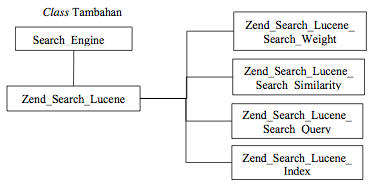
\includegraphics[width=200pt]{class.png}
\caption{Struktur penggunaan \textit{class}}
\label{fig:class}
\end{figure}

\textit{Class} \textbf{Search\textunderscore Engine} memiliki fungsi sebagai berikut:
\begin{enumerate}[noitemsep] 
\item \textbf{indexing()}, digunakan untuk melakukan fungsi indexing
\item \textbf{getManfaat()}, digunakan untuk parsing data RDF pada field manfaat dengan tipe data $<$rdf:Bag$>$
\item \textbf{getKandungan()}, digunakan untuk parsing data RDF pada field kandungan
dengan tipe data $<$rdf:Bag$>$
\item \textbf{doSearch}, digunakan untuk melakukan proses pencarian
\end{enumerate}

Pengguna memasukkan kueri yang selanjutnya akan diproses oleh fungsi \textbf{doSearch} yang terdapat pada \textit{class} \textbf{Search\textunderscore engine}. Fungsi \textbf{doSearch} dijalankan ketika terdapat kueri yang ingin dicari di dalam koleksi dokumen RDF. Fungsi \textbf{doSearch} yang selanjutnya diproses melalui \textit{search engine} Lucene. Setelah kueri diproses Lucene akan menemukembalikan dokumen yang relevan berdasarkan ranking tertinggi.

Untuk melakukan \textit{indexing}, dokumen RDF yang akan diindeks disimpan dalam sebuah aplikasi penyimpanan dokumen RDF yaitu Sesame. Proses \textit{indexing} dilakukan oleh fungsi \textbf{indexing()} yang terdapat pada \textit{class} \textbf{Search\textunderscore engine}. Fungsi \textbf{indexing()} akan melakukan \textit{parsing} data dokumen RDF pada media penyimpanan Sesame dengan menggunakan kueri SPARQL. Hasil \textit{parsing} data selanjutnya akan diindeks melalui \textit{search engine} Lucene. Hasil \textit{indexing} akan disimpan pada \textit{folder} \textbf{tmp/rdf-indeks} yang terdapat pada direktori \textbf{/xampp/htdocs/Lucene/}.

\subsection*{Pencarian}
Setelah dilakukan proses \textit{indexing}, maka dapat dilakukan pencarian pada dokumen RDF tanaman obat. Pencarian dilakukan dengan memasukkan kueri pada sistem \textit{search engine}. Jumlah kueri yang digunakan pada penelitian ini adalah 29 kueri. Kueri pada sistem ini dapat berupa kata tunggal, frase, dan gabungan dari \textit{field} yang dipilih dengan kata tunggal atau frase. Kueri akan diproses oleh sistem Lucene yang akan me-\textit{retrieve} dokumen yang relevan beserta skoringnya. Pada Lucene, jika hasil skoring lebih besar dari 1.0 maka nilai skoring akan dibulatkan menjadi 1.0. Tabel \ref{tab:hasilkueri} ditunjukkan hasil temu kembali terhadap dokumen RDF tanaman obat.

\begin{table}[h!]
\footnotesize
\caption{Hasil temu kembali dokumen RDF tanaman obat}
\centering
\begin{tabulary}{0.47\textwidth}{RLRR}
\toprule
No.&\parbox{8em}{Kueri} & \textit{Retrieved} & Relevan \\
\midrule
1. & Kanker & 3 & 3\\
2.&Flu&2&2\\
3.&Diabetes&17&17\\
4.&Pusing&3&3\\
5.&Merambat&1&1\\
6.&Menjari&2&2\\
7.&Bergerigi&15&11\\
8.&Menyirip&19&14\\
9.&Vitamin&16&15\\
10.&Antioksidan&1&1\\
11.&Protein&6&3\\
12.&Kalsium&13&8\\
13.&Diseduh&12&11\\
14.&Ditumbuk&13&12\\
15.&Diperas&7&7\\
16.&Batuk Pilek&27&3\\
17.&Kencing Batu&47&4\\
18.&Datang Bulan&13&3\\
19.&Gatal-gatal&11&4\\
20.&Sesak Nafas&9&6\\
\bottomrule
\end{tabulary}
\label{tab:hasilkueri}
\end{table}

Kueri ditentukan dengan cara memilih kata tunggal atau frase yang mewakili isi setiap tanaman obat. Kata-kata tersebut berkaitan dengan penyakit yang dapat disembuhkan, kandungan kimia, karakter fisik, dan cara penggunaan tanaman obat. Pada Lucene disediakan fitur \textit{term boosting} yang dapat meningkatkan tingkat akurasi hasil temu kembali informasi. Pada penelitian ini, tiga kueri yang memiliki tingkat akurasi yang rendah diberikan \textit{term boosting} seperti pada Tabel \ref{tab:hasilboosting}.

\begin{table}[h!]
\footnotesize
\caption{Kueri dengan \textit{term boosting}}
\centering
\begin{tabulary}{0.47\textwidth}{RLRR}
\toprule
No.&\parbox{8em}{Kueri} & \textit{Retrieved} & Relevan \\
\midrule
1. & obat diseduh(4)&42&4\\
2. & obat ditumbuk(4)&39&8\\
3. & buah diperas(4)&60&3\\ 
\bottomrule
\end{tabulary}
\label{tab:hasilboosting}
\end{table}

\subsection*{Evaluasi}
Evaluasi kinerja search engine dilakukan menggunakan nilai interpolasi maksimum \textit{recall} dan \textit{precision}. Pengujian dilakukan terhadap 29 kueri berupa kata tunggal atau frase dan dokumen yang relevan. Setiap kueri akan dihitung nilai \textit{precision} pada setiap nilai \textit{recall} standar yatu 0, 0.1, 0.2, 0.3, 0.4, 0.5, 0.6, 0.7, 0.8, 0.9, 1.0. Setelah didapatkan nilai \textit{precision} pada sebelas nilai \textit{recall} untuk setiap kueri, kemudian dicari nilai interpolasi maksimum \textit{recall} dan \textit{precision}. Nilai interpolasi maksimum \textit{recall} dan \textit{precision} dapat dilihat pada Gambar \ref{fig:recall}.
\begin{figure}[h!]\centering 
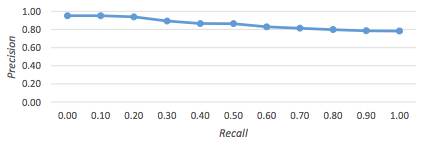
\includegraphics[width=200pt]{recall.png}
\caption{Rataan \textit{recall precision} dengan interpolasi maksimum}
\label{fig:recall}
\end{figure}

Dari percobaan yang dilakukan terhadap 29 kueri didapatkan nilai \textit{precision} sebesar 0.862. Dapat disimpulkan bahwa kinerja sistem temu kembali informasi memiliki tingkat keakuratan yang baik untuk semua kueri yang diberikan.

Dokumen yang tidak relevan tetapi tetap ditemukembalikan terjadi pada kueri ‘Batuk Pilek’, ‘Kencing Batu’, ‘Datang Bulan’, ‘Gatal-gatal’, ‘Buah Diperas’, ‘Tanaman Hias’, ‘Tumbuhan Merambat’, ‘Daun Elips’, ‘Buah Buni’, ‘Kalsium Oksalat, ‘Zat Warna’, ‘Obat Diseduh’, dan ‘Obat Ditumbuk. Hal ini disebabkan karena kueri tersebut memiliki banyak arti dalam setiap dokumen tanaman obat, sehingga tidak mampu mewakili informasi yang diinginkan pengguna. Misalnya pada kueri ‘Tumbuhan Merambat’ informasi yang diinginkan pengguna adalah mengenai tanaman obat yang tumbuh merambat, tetapi sistem akan menemukembalikan dokumen yang mengandung kata ‘Tumbuhan’ dan ‘Merambat’. Hal tersebut yang mempengaruhi nilai \textit{precision} yang didapat pada penelitian ini. Hal ini terbukti dengan menghilangkan kueri dua kata mengakibatkan perubahan nilai \textit{recall} dan \textit{precision} seperti terlihat pada Gambar \ref{fig:boosting}.
\begin{figure}[h!]\centering 
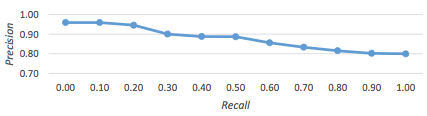
\includegraphics[width=200pt]{boosting1.png}
\caption{\textit{Recall precision} untuk kueri kata tunggal}
\label{fig:boosting}
\end{figure}

\vfill\eject % memaksa pindah kolom/halaman
Untuk kueri dengan dua kata, perlu ditambahkan penguatan pada kata tertentu dengan menggunakan \textit{term boosting} agar sistem dapat mengetahui kata yang dipentingkan. Dengan menambahkan \textit{term boosting}, nilai rataan \textit{precision} yang didapatkan lebih baik yaitu 0.877. Pada evaluasi ini juga dilakukan perhitungan \textit{recall} dan \textit{precision} dengan menggunakan nilai \textit{term boosting} yang berbeda pada masing-masing kueri yang menggunakan dua kata yaitu ‘Obat Diseduh(6)’, ‘Obat Ditumbuk(6)’, dan ‘Buah Diperas(6)’. Nilai \textit{recall} dan \textit{precision} yang dihasilkan setelah nilai \textit{term boosting} ditambahkan dapat dilihat pada Gambar \ref{fig:boosting2}.
\begin{figure}[h!]\centering 
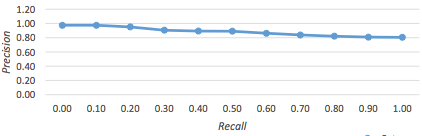
\includegraphics[width=200pt]{boosting2.png}
\caption{\textit{Recall precision} dengan \textit{term boosting}}
\label{fig:boosting2}
\end{figure}

Nilai rataan precision yang dihasilkan dengan penambahan nilai \textit{term boosting} yaitu 0.884. Dari Gambar \ref{fig:boosting2} dapat terlihat bahwa kueri dengan menambahkan \textit{term boosting} yang makin tinggi sampai pada nilai tertentu dapat meningkatkan keakuratan hasil temukembali informasi.

\subsection*{Contoh Penulisan Algoritme}
Bagian ini adalah tambahan penulisan untuk mengetahui cara menuliskan algoritme yang diacu maupun yang tidak diacu dalam teks. Algoritme \ref{algo:max} dibuat untuk mendapatkan bilangan terbesar dari kumpulan bilangan yang terhingga.
\begin{algorithm}
\DontPrintSemicolon % Some LaTeX compilers require you to use \dontprintsemicolon instead
\KwIn{Himpunan $A=\{a_1, a_2, \ldots, a_n\}$}
\KwOut{Bilangan terbesar}
$max \gets a_1$\;
\For{$i \gets 2$ \textbf{to} $n$} {
  \If{$a_i > max$} {
    $max \gets a_i$\;
  }
}
\Return{$max$}\;
\caption{{\sc Max} mendapatkan bilangan terbesar}
\label{algo:max}
\end{algorithm}

\vfill\eject % memaksa pindah kolom/halaman
\noindent Berikut adalah algoritme tanpa referensi dan caption, yang tidak diacu dalam teks:
\begin{algorithm}
\DontPrintSemicolon % Some LaTeX compilers require you to use \dontprintsemicolon instead 
\KwIn{A set $C = \{c_1, c_2, \ldots, c_r\}$ of denominations of coins, where $c_i > c_2 > \ldots > c_r$ and a positive number $n$}
\KwOut{A list of coins $d_1,d_2,\ldots,d_k$, such that $\sum_{i=1}^k d_i = n$ and $k$ is minimized}
$C \gets \emptyset$\;
\For{$i \gets 1$ \textbf{to} $r$}{
  \While{$n \geq c_i$} {
    $C \gets C \cup \{c_i\}$\;
    $n \gets n - c_i$\;
  }
}
\Return{$C$}\;
\end{algorithm}


%----------------------------------------------------------------------------------------
%	BAGIAN KESIMPULAN
%----------------------------------------------------------------------------------------

%----------------------------------------------------------------------------------------
%	KESIMPULAN DAN SARAN
%----------------------------------------------------------------------------------------
\section*{KESIMPULAN DAN SARAN}
\subsection*{Kesimpulan}
Pada penelitian ini dapat disimpulkan bahwa:
\begin{enumerate}[noitemsep]
\item Mesin pencari menggunakan Lucene pada dokumen RDF dapat dilakukan. Lucene tidak dapat secara langsung mengolah dokumen RDF karena dokumen RDF harus disimpan dan diolah menggunakan Sesame.
\item Hasil pencarian yang dilakukan menggunakan 29 kueri yang didapat dari penelitian \citeauthor{HERAWAN} (\cite*{HERAWAN}) menghasilkan nilai rataan \textit{precision} yang baik yaitu 0.862 dan menggunakan kueri dengan \textit{term boosting} menghasilkan nilai rataan \textit{precision} 0.877.
\item Penambahan nilai \textit{term boosting} menghasilkan nilai rataan precision 0.884.
\item Dokumen XML dapat dikonversi menjadi dokumen RDF. Agar dokumen RDF yang dihasilkan memiliki struktur yang jelas, maka dilakukan konversi secara manual.
\end{enumerate}

\subsection*{Saran}
Terdapat beberapa hal yang dapat ditambahkan atau diperbaiki untuk penelitian selanjutnya, yaitu:
\begin{enumerate}[noitemsep]
\item Jumlah dokumen tanaman obat yang digunakan sebagai korpus diperbanyak lagi, agar pengukuran relevansi dapat dilakukan lebih jelas.
\item Menggunakan ontologi untuk dokumen RDF agar makna dari informasi pada dokumen RDF dapat lebih spesifik.
\end{enumerate}


%----------------------------------------------------------------------------------------
%	BAGIAN DAFTAR PUSTAKA
%----------------------------------------------------------------------------------------

\renewcommand{\refname}{DAFTAR PUSTAKA}
\nocite{*}
\printbibliography

%----------------------------------------------------------------------------------------

\end{document}